\chapter{Resultats dels tests}
\label{appendix-results}
A continuaci� es mostren els gr�fics amb la resta de resultats de les proves que s'han realitzat. La majoria corresponen al mateix tipus de tests que els del cap�tol \ref{chapter:results}, per� variant algun par�metre.

\section{Cerca de refer�ncies}
Les gr�fiques seg�ents s�n semblants a la de la figura \ref{fig:results:random-reslen}. En aquest cas, per�, el tipus de fitxers per als quals extraiem consultes i fem les cerques estan agrupats en dues categories segons l'estructura del seu contingut. Per un costat, a la figura \ref{fig:results:pageheader-reslen}, tenim fitxers que tenen una p�gina sencera com a cap�alera abans del resum o \textit{abstract} de l'article.
\begin{figure}[H]
\begin{center}
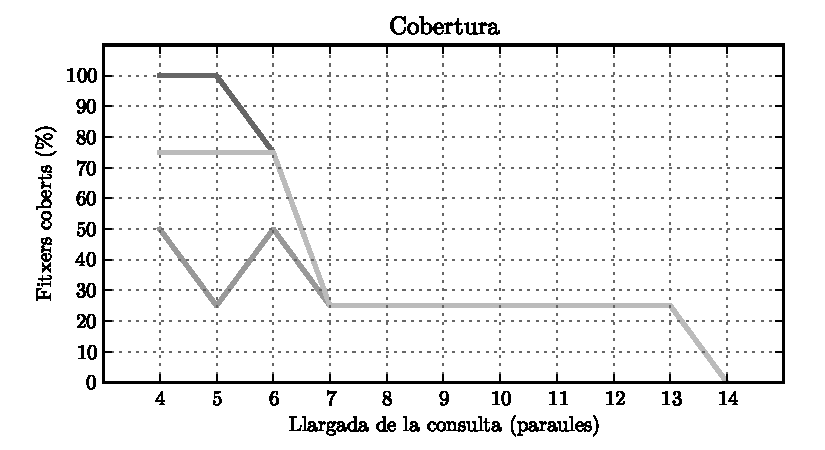
\includegraphics[width=0.8\textwidth]{figures/results:pageheader-reslen.pdf}
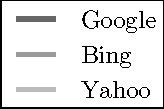
\includegraphics[scale=0.8]{figures/results:search-legend.pdf}
\caption{Qualitat dels resultats per fitxers amb una p�gina sencera com a cap�alera}
\label{fig:results:pageheader-reslen}
\end{center}
\end{figure}

Veiem que per aquest tipus d'article, el percentatge de p�gines per les quals s'han obtingut bons resultats disminueix molt a mesura que s'augmenta la llargada de la consulta. Cal tenir en compte que les consultes s'han obtingut totes a partir de la primera p�gina del fitxer. Al no contenir el resum, fa que l'expressi� regular usada per trobar la consulta no tingui coincid�ncies per la majoria dels articles provats. Si executem les mateixes proves, per� agafant les consultes de les dues primeres p�gines, els resultats milloren for�a:

\begin{figure}[H]
\begin{center}
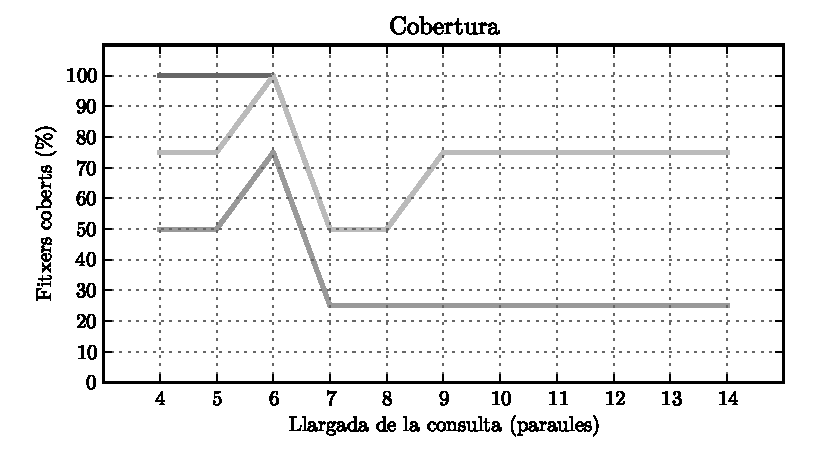
\includegraphics[width=0.8\textwidth]{figures/results:pageheader2-reslen.pdf}
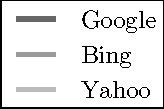
\includegraphics[scale=0.8]{figures/results:search-legend.pdf}
\caption{Qualitat dels resultats per fitxers amb una p�gina sencera com a cap�alera II}
\label{fig:results:pageheader2-reslen}
\end{center}
\end{figure}

El gr�fic de la figura seg�ent s'ha obtingut a partir d'articles que tenen una cap�alera \textit{normal}. Considerem que les cap�aleres dels articles m�s habituals s�n aquelles que tenen l'\textit{abstract} a la mateixa p�gina.
\begin{figure}[H]
\begin{center}
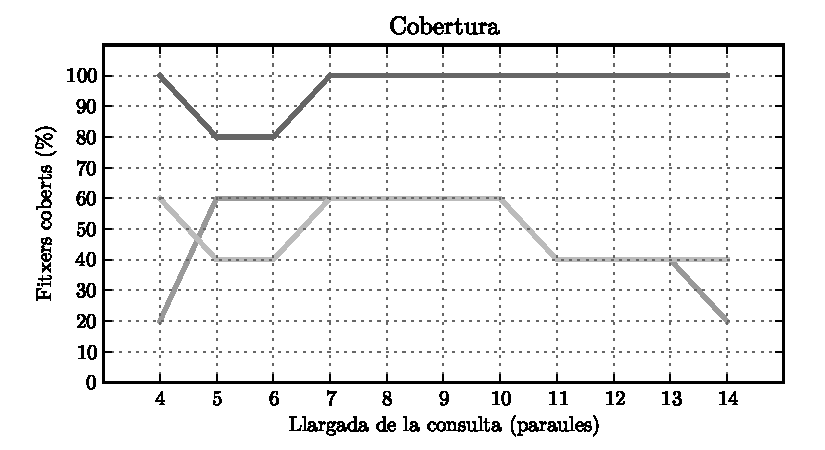
\includegraphics[width=0.8\textwidth]{figures/results:usualheader-reslen.pdf}
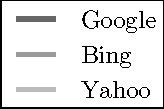
\includegraphics[scale=0.8]{figures/results:search-legend.pdf}
\caption{Qualitat dels resultats per fitxers amb cap�aleres \textit{normals}}
\label{fig:results:usualheader-reslen}
\end{center}
\end{figure}

\paragraph{}
Pel que fa al n�mero de consultes necess�ries per comen�ar a obtenir bons resultats, els gr�fics per aquests dos conjunts de fitxers s�n molt semblants al que hem vist a la figura \ref{fig:results:random-fqlen}.

\section{Generaci� de \textit{wrappers}}
\label{appendix:results:section:wrapperinduction}
Pel que fa a la generaci� autom�tica de regles d'extracci�, la figura seg�ent mostra els \textit{wrappers} obtinguts al generar-los fent servir nom�s dos exemples. Com es pot comprovar,
A continuaci� es mostren els gr�fics de la cobertura dels \textit{wrappers} generats per altres camps que no s'han tractat a la secci� \ref{chapter:results:section:wrapperinduction}.


\begin{figure}[H]
\begin{center}
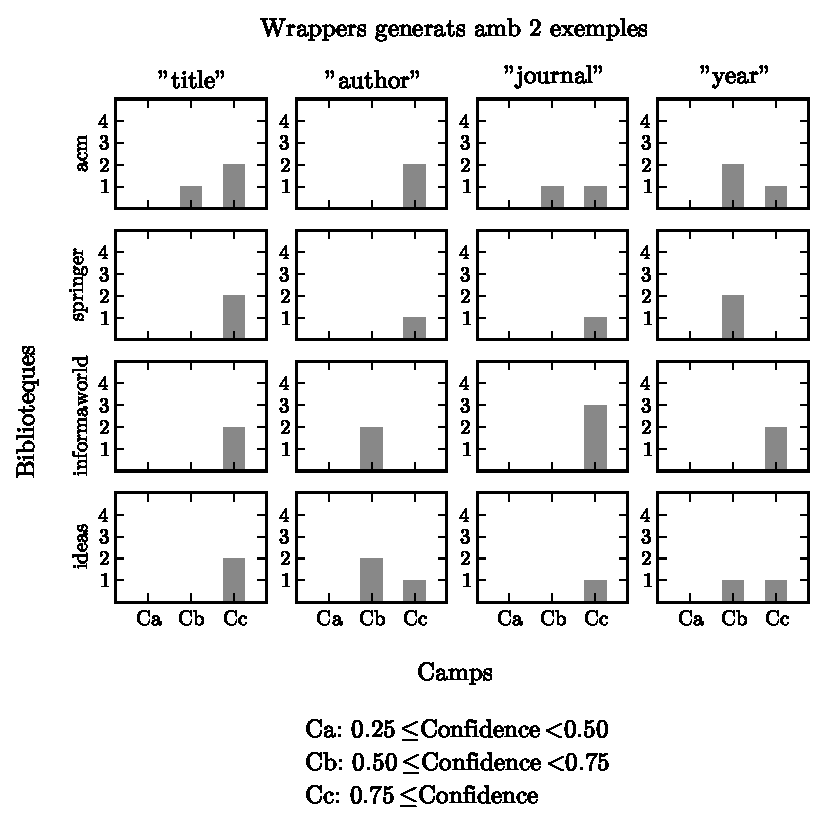
\includegraphics[width=0.8\textwidth]{figures/results:nwrappers-2.pdf}
\caption{Nombre de \textit{Wrappers} generats utilitzant 2 exemples i agrupats per confian�a}
\label{fig:results:nwrappers-2}
\end{center}
\end{figure}


\begin{figure}[H]
\begin{center}
\begin{minipage}{0.49\linewidth}
	\centering
	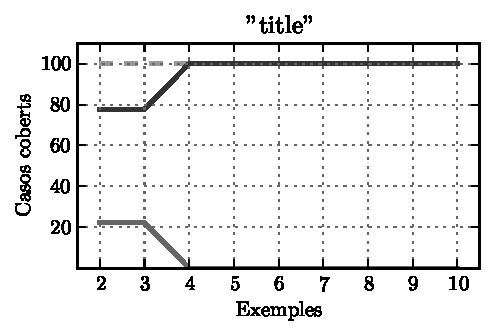
\includegraphics[width=\textwidth]{figures/results:coverage-title.pdf}
\end{minipage}
\hspace{0cm}
\begin{minipage}{0.49\linewidth}
	\centering
	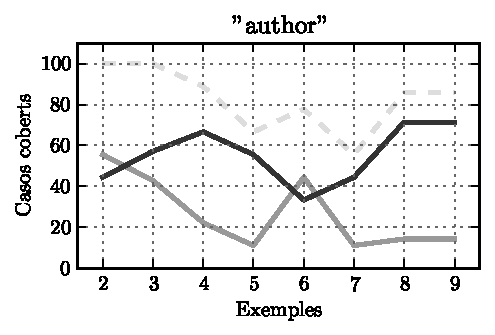
\includegraphics[width=\textwidth]{figures/results:coverage-author.pdf}
\end{minipage}
\end{center}
\end{figure}

\begin{figure}[H]
\begin{center}
\begin{minipage}{0.49\linewidth}
	\centering
	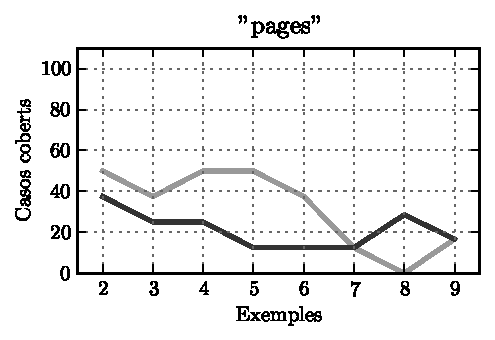
\includegraphics[width=\textwidth]{figures/results:coverage-pages.pdf}
\end{minipage}
\hspace{0cm}
\begin{minipage}{0.49\linewidth}
	\centering
	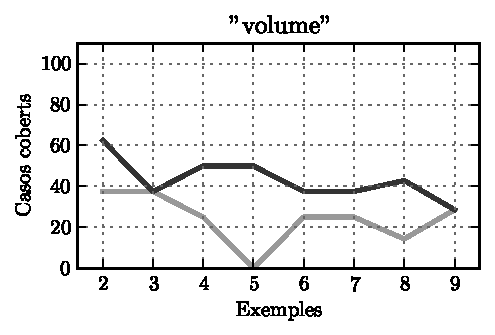
\includegraphics[width=\textwidth]{figures/results:coverage-volume.pdf}
\end{minipage}

\begin{minipage}{\linewidth}
	\centering
	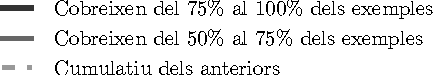
\includegraphics{figures/results:coverage-legend.pdf}
\end{minipage}

\caption{Cobertura dels \textit{wrappers} generats}
\label{fig:appendix:results:wrapperinduction:coverage}
\end{center}
\end{figure}



\begin{figure}[H]
\begin{center}
	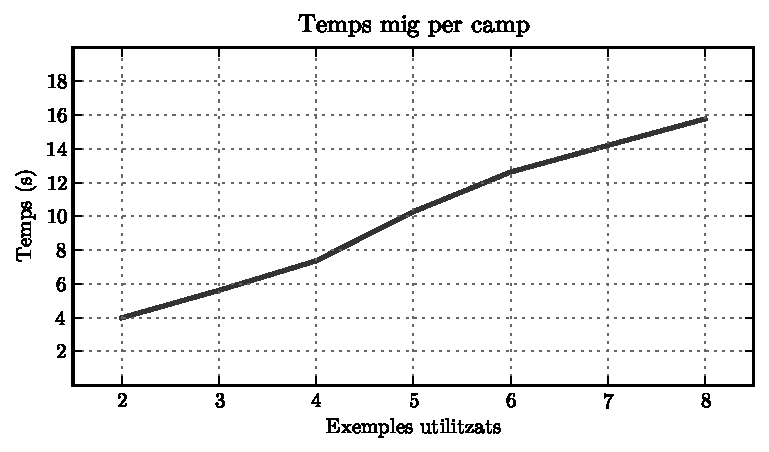
\includegraphics[width=0.8\textwidth]{figures/results:field-time.pdf}
	\caption{Temps mitj� per la generaci� dels \textit{wrappers} d'un �nic camp}
	\label{fig:appendix:results:wrapperinduction:time}
\end{center}
\end{figure}
	


